\cotefile{154}
\scanpage{46}
% archive sheet number: 45

inverses des $D_i$ dans $\widetilde X$. (à ne pas confondre avec les revêtements des bords des $D_i$, quand on n'a pas choisi d'orientation de $D_i$)

\textcircled{$i$} On a une application

\[ \mathcal X \xrightarrow{\varphi} Y. \]

(application structurale) \inserted{quelles \deleted{\unsure{con}}ditions}

2) La restriction de $\varphi$ à \deleted{tt} face de $(\mathcal X,K)$ est un \deleted{\unsure{polygone}} \inserted{isomor\unsure{.}} \unsure{telle que}

% slanted
\margin{\unsure{Donc} \unsure{sauf les} \deleted{qu'elle construite} \deleted{en 2 \unsure{principes}} pour faces exceptionnelles, pour certaines arêtes, en un point !}

\deleted{1) L'ensemble $\Sigma$ \unsure{pte} à \unsure{$\varphi$ est fini} \unsure{$\mathrm{id}_{\mathcal X}$} $\mathcal X\smallsetminus K$}

Au voisinage de l'un \deleted{de tt point de $K\smallsetminus S(K)$,} \inserted{des bords de $K$,} $\varphi$ a la structure d'un ``folding'' d'arête.

3) Au voisinage de tt \deleted{pt} sommet de $K$, $\varphi$ a la structure d'un ``double folding'' relatif : $s$ et les deux branches de $K$ passant en $s$

4) \deleted{L'image \unsure{p} de tt sommet de $L$} \deleted{On a} \deleted{$\varphi^{-1}(\bigcup D_i)\cap K=\unsure{S}(L)\cap$} \deleted{($\Longrightarrow\varphi^{-1}(X_1)\cap K$} \quad $L=\varphi^{-1}(\underbrace{\bigcup D_i}_{X_1\deleted{\unsure{X_2}}})$

\margin{Considéré tel quel, il faut se placer en dehors des ``\unsure{endroits|environs}'' autour des composantes de $K_0$}

Cor. \inserted{pour} \unsure{tt} pt de $s\in K\cap\unsure{\vphantom L'|{}}L=(\varphi\mid K)^{-1}(X_1)$, \deleted{\illegible{1} est un} $\varphi(s)$ est un sommet, ssi \deleted{$s$ est un sommet de} \inserted{n'est \uline{pas} un sommet de $K$, et est un sommet de $L$} \deleted{la carac. est le sommet critique de} --- i.e. est un \uline{point critique} de $K$. (l'\unsure{ens.} de ces pts est en corr. 1-1 avec l'ens des arêtes ordinaires de $K$).

\deleted{\unsure{j)} Soit.} j) Soit $F$ une face de $(\mathcal X,K)$. Considérons les \deleted{\unsure{éléments}} \inserted{pts} critiques de $K$ en $\partial F$, tels que la branche marquée en \deleted{\unsure{un sommet}} \inserted{$s$ (cf (d))} \deleted{\unsure{ou}} soit extérieure à $F$, et corrigeons le contour $\partial F$ par un petit renflement \deleted{de sorte que} \inserted{de façon} à ce que $s$ soit du côté privilégié de $s$.

\figure{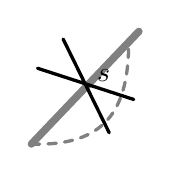
\begin{tikzpicture}[scale=.65,line cap=round]
\draw[line width=2.7pt,gray] (-1.1,-1.05)--(1,1.15);
\draw[gray,very thick,dashed] (-1.1,-1.05) .. controls (.35,-1.1) and (.8,-.38) .. (.8,.93);
\draw[very thick] (-.98,.43)--(.9,-.18) (-.48,1)--(.42,-.83);
\node at (.31,.29) {$s$};
\end{tikzpicture}}

% slanted
\margin{\uline{NB} \uline{(pour j)} Supposons pour \deleted{le voir} \unsure{seulement même} i.e. \unsure{$\exists$} un pt critique $s$ est sur le voisin privilégié, \unsure{en face de|une face} $F$ il \deleted{suffit} et s. que les \unsure{deux} \uline{branches de $L$} passant par $s$ se recoupent toutes en un autre point du bord de $F$ (dans le cas contraire, \deleted{les \unsure{autres deux}} qu'une au moins des deux branches sur le bord de $F$ sont \unsure{trid\textsuperscript{les}|toutes deux} et se rencontrent \unsure{cf} $F$ et $F'$ ci dessous}

\figure{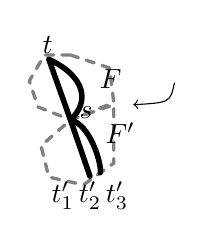
\begin{tikzpicture}[scale=.55,line join=round,line cap=round]
\draw[gray,very thick,dashed] (0,2)--(.9,1.7)--(1,.9)--(0,.5)--(-.75,.8)--(-.95,1.4)--(-.6,2)--cycle;
\draw[gray,very thick,dashed] (0,.5)--(1,.85)--(1,-.5)--(.3,-1)--(-.5,-.82)--(-.68,-.1)--cycle;
\draw[line width=2pt] (-.5,1.9)--(0,.5)--(.45,-.8) (-.5,1.9) .. controls (.35,1.5) and (.45,.92) .. (0,.5) .. controls (.45,.4) and (.72,-.5) .. (.69,-.72);
\node at (-.53,2.22){$t$};\node at (.36,.66){$s$};\node at (.93,1.45){$F$};\node at (1.15,.2){$F'$};\node at (.45,-1.25){$t'_1\,t'_2\,t'_3$};\draw[->] (2.4,1.35) .. controls (2.3,.9) .. (1.45,.85);
\end{tikzpicture}}

Soit \deleted{$\partial\unsure{F}$} $F'$ \deleted{\unsure{sa} la face \unsure{fermée}} \inserted{($F'\supset F$)} \deleted{\unsure{on trouve}} \inserted{on désigne} alors \deleted{\unsure{alors}} la position relative correspondante : $\mathcal F$ est $\varphi(\partial' F)$, et \deleted{elle est} le système affine correspondant est canoniquement \deleted{isomorphe par} \inserted{isomorphe à} \deleted{$F',\unsure{\mathcal F}$} $(F',F'\cap L)$.

k) Appelons une arête exceptionnelle \uline{stable} ou instable (ou semi-stable) suivant que les deux \deleted{positions relatives} \inserted{faces} incidentes correspondantes : des pr. stables (resp. instables) (contiennent chacune resp. cont. \unsure{aucun}). Alors pour \deleted{\unsure{tout}} un sommet exceptionnel les bords privilégiés de la branche ord. de $K$ qui y passe est du côté de l'arête exc. instable (côté \unsure{fermé})
